
% This LaTeX was auto-generated from MATLAB code.
% To make changes, update the MATLAB code and republish this document.

\documentclass{article}
\usepackage{graphicx}
\usepackage{color}
\usepackage{amsmath}
\usepackage{amssymb}
\usepackage[a4paper, total={6in,8in}]{geometry}
\usepackage{pdfpages}
\usepackage{multicol}

\sloppy
\definecolor{lightgray}{gray}{0.5}
\setlength{\parindent}{0pt}

\begin{document}

\includepdf{../TitlePage.pdf}

\hrulefill
\section*{\#1(a)}

\begin{verbatim}
clear;clc;close all
[x, y] = meshgrid(0:0.01:1,0:0.01:1);
len = size(x);
for i = 1:len(1)
    for j = 1:len(2)
        f = @(m) (sinh((2*m-1)*pi*(1-y(i,j)))+sinh((2*m-1)*pi*y(i,j)))/sinh((2*m-1)*pi) ...
        *sin((2*m-1)*pi*x(i,j))/(2*m-1)^3;
        T(i,j) = (x(i,j)^2-x(i,j))/2 + 4/pi^3*limsum(f);
    end
end

figure()
surf(x,y,T, 'edgecolor', 'none')
title("$\frac{q_0}{2}(x^2-x)+\frac{4q_0}{\pi^3}\sum\limits^{\infty}_{m=1,3,5,...} ...
\frac{1}{m^3}[\frac{\sinh{m\pi(1-y)}+\sinh{m\pi y}}{\sinh{m\pi}}]\sin{m\pi x}$ 3D Plot", ...
"fontsize", 14, 'interpreter', 'latex')

figure()
contour(x,y,T,'ShowText','on')
title("$\frac{q_0}{2}(x^2-x)+\frac{4q_0}{\pi^3}\sum\limits^{\infty}_{m=1,3,5,...} ...
\frac{1}{m^3}[\frac{\sinh{m\pi(1-y)}+\sinh{m\pi y}}{\sinh{m\pi}}]\sin{m\pi x}$ 2D Plot", ...
"fontsize", 14, 'interpreter', 'latex')
\end{verbatim}

\dotfill
\begin{figure}[h!]
    \begin{multicols}{2}
        \includegraphics [width=3in]{HW3_01.png}
        \columnbreak

        \includegraphics [width=3in]{HW3_02.png}
    \end{multicols}
\end{figure}


\hrulefill
\section*{\#1(b)}

\begin{verbatim}
clear;clc;close all
[x, y] = meshgrid(0:0.01:1,0:0.01:1);
len = size(x);
for i = 1:len(1)
    for j = 1:len(2)
        tamp = 0;
        f = @(n,m) sin((2*m-1)*pi*x(i,j))*sin((2*n-1)*pi*y(i,j))/((2*m-1)*(2*n-1) ...
        *(((2*m-1)*pi)^2+((2*n-1)*pi)^2));
        for n = 1:100
            for m = 1:100
                tamp = tamp + f(n,m);
            end
        end
        T(i,j) = -16/pi^2*tamp;
    end
end

figure()
surf(x,y,T, 'edgecolor', 'none')
title("$\frac{-16q_0}{\pi^2}\sum\limits^{\infty}_{m=1,3,5,...}\sum\limits ...
^{\infty}_{n=1,3,5,...}\frac{1}{mn[(m\pi)^2+(n\pi)^2]}\sin{m\pi x}\sin{n\pi y}$ 3D Plot" ...
, "fontsize", 14, "interpreter", "latex")

figure()
contour(x,y,T,'ShowText','on')
title("$\frac{-16q_0}{\pi^2}\sum\limits^{\infty}_{m=1,3,5,...}\sum\limits ...
^{\infty}_{n=1,3,5,...}\frac{1}{mn[(m\pi)^2+(n\pi)^2]}\sin{m\pi x}\sin{n\pi y}$ 2D Plot" ...
, "fontsize", 14, "interpreter", "latex")
\end{verbatim}

\dotfill
\begin{figure}[h!]
    \begin{multicols*}{2}
        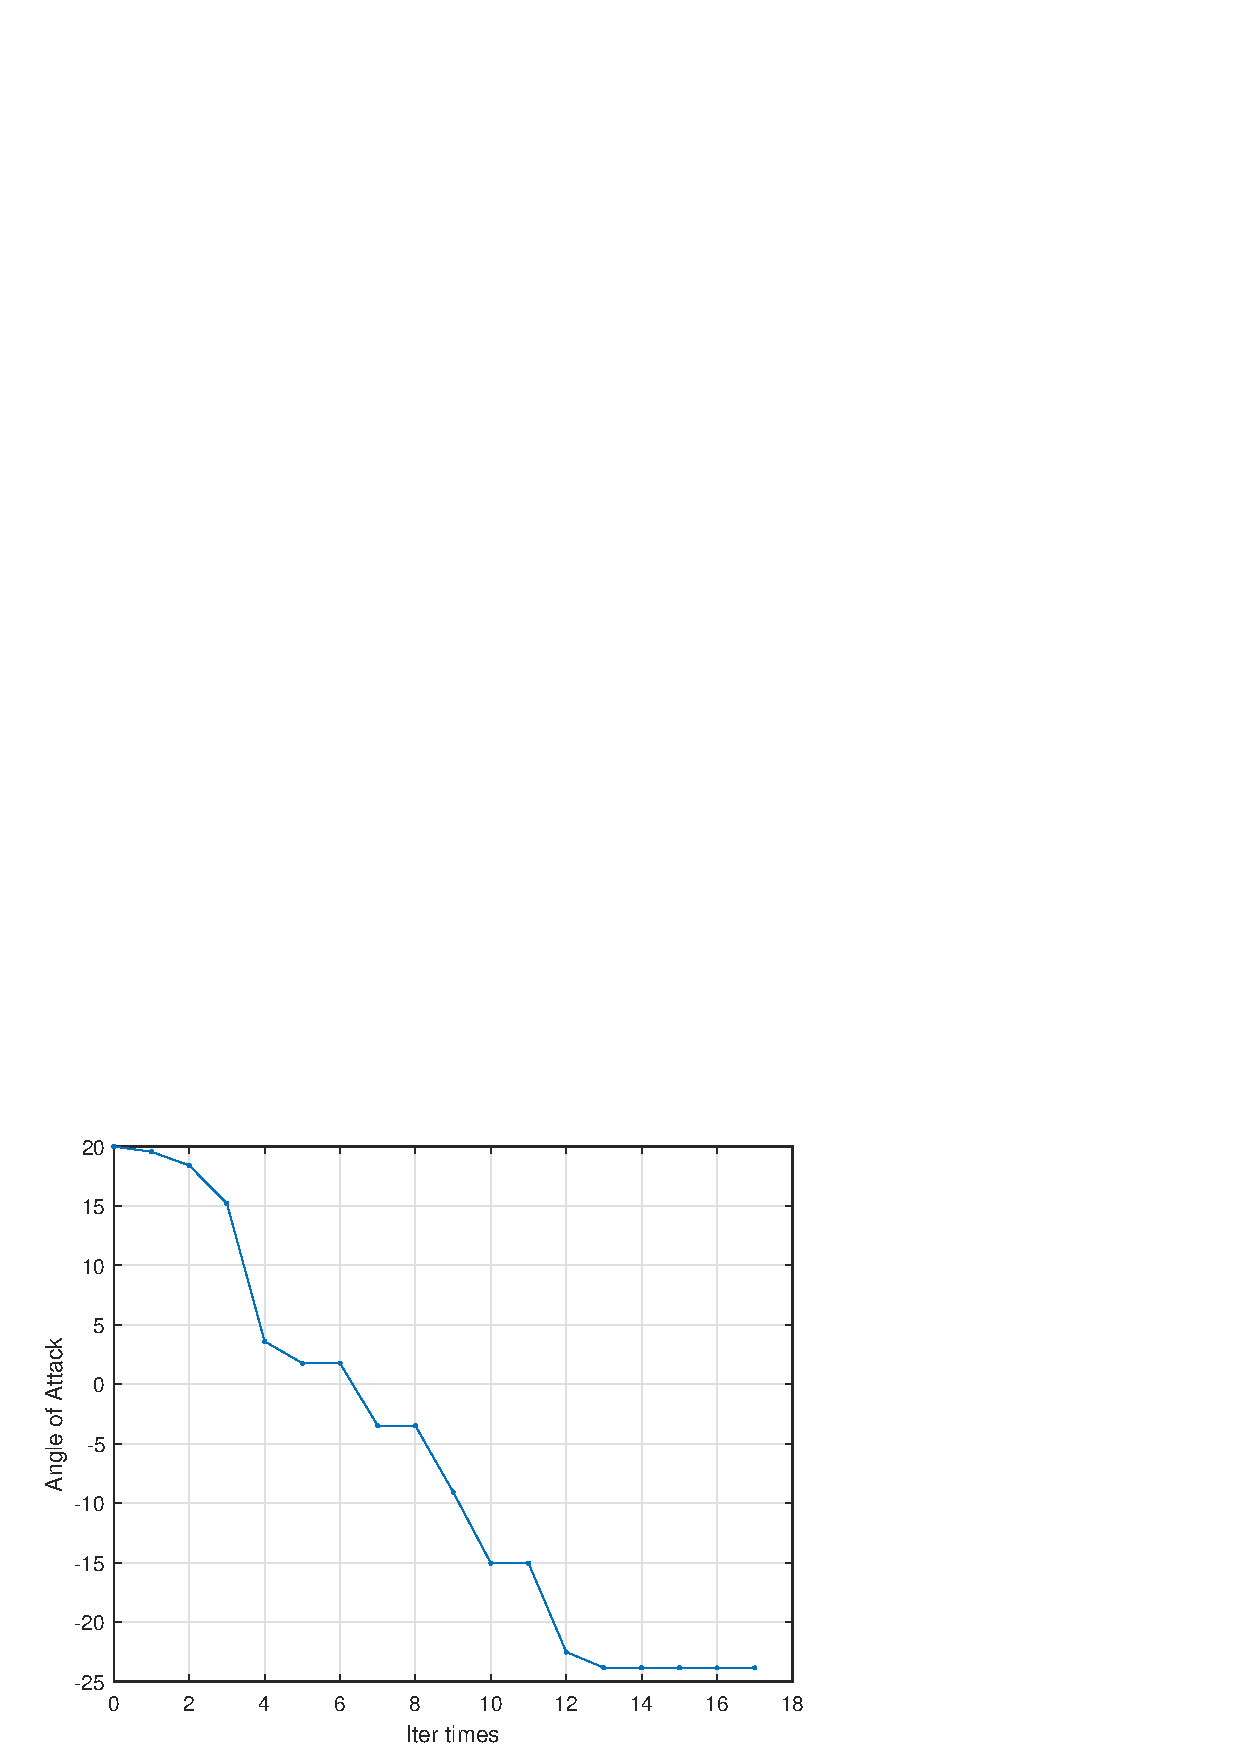
\includegraphics [width=3in]{HW3_03.png}
        \columnbreak

        \includegraphics [width=3in]{HW3_04.png}
    \end{multicols*}
\end{figure}

\hrulefill
\section*{\#2(a)}

\begin{verbatim}
clear;clc;close all
[x, y] = meshgrid(0:0.01:1,0:0.01:1);
phi_12 = sin(1*x).*sin(2*y);
phi_21 = sin(2*x).*sin(1*y);
phi_13 = sin(1*x).*sin(3*y);
phi_31 = sin(3*x).*sin(1*y);

figure()
surf(x,y,phi_12, 'edgecolor', 'none')
title("$\phi_{12}$ 3D Plot", "fontsize", 14, "interpreter", "latex")
figure()
surf(x,y,phi_21, 'edgecolor', 'none')
title("$\phi_{21}$ 3D Plot", "fontsize", 14, "interpreter", "latex")

figure()
contour(x,y,phi_12,'ShowText','on')
title("$\phi_{12}$ 2D Plot", "fontsize", 14, "interpreter", "latex")
figure()
contour(x,y,phi_21,'ShowText','on')
title("$\phi_{21}$ 2D Plot", "fontsize", 14, "interpreter", "latex")
\end{verbatim}

\dotfill
\begin{figure}[h!]
    \begin{multicols*}{2}
        \includegraphics [width=3in]{HW3_05.png}

        \includegraphics [width=3in]{HW3_06.png}

        \includegraphics [width=3in]{HW3_07.png}

        \includegraphics [width=3in]{HW3_08.png}
    \end{multicols*}
\end{figure}
\newpage


\hrulefill
\section*{\#2(b)(c)(d)(e)}

\begin{verbatim}
clear;clc;close all
[x, y] = meshgrid(0:0.01:1,0:0.01:1);
phi_12 = sin(1*x).*sin(2*y);
phi_21 = sin(2*x).*sin(1*y);
phi_13 = sin(1*x).*sin(3*y);
phi_31 = sin(3*x).*sin(1*y);

figure()
surf(x,y,phi_12+phi_21, 'edgecolor', 'none')
title("$\phi_{12}+\phi_{21}$ 3D Plot", "fontsize", 14, "interpreter", "latex")
figure()
surf(x,y,phi_13+phi_31, 'edgecolor', 'none')
title("$\phi_{13}+\phi_{31}$ 3D Plot", "fontsize", 14, "interpreter", "latex")
figure()
surf(x,y,phi_13-phi_31, 'edgecolor', 'none')
title("$\phi_{13}-\phi_{31}$ 3D Plot", "fontsize", 14, "interpreter", "latex")
figure()
surf(x,y,phi_13+phi_31/3, 'edgecolor', 'none')
title("$\phi_{13}+\frac{1}{3}\phi_{31}$ 3D Plot", "fontsize", 14, "interpreter", "latex")

figure()
contour(x,y,phi_12+phi_21,'ShowText','on')
title("$\phi_{12}+\phi_{21}$ 2D Plot", "fontsize", 14, "interpreter", "latex")
figure()
contour(x,y,phi_13+phi_31,'ShowText','on')
title("$\phi_{13}+\phi_{31}$ 2D Plot", "fontsize", 14, "interpreter", "latex")
figure()
contour(x,y,phi_13-phi_31,'ShowText','on')
title("$\phi_{13}-\phi_{31}$ 2D Plot", "fontsize", 14, "interpreter", "latex")
figure()
contour(x,y,phi_13+phi_31/3,'ShowText','on')
title("$\phi_{13}+\frac{1}{3}\phi_{31}$ 2D Plot", "fontsize", 14, "interpreter", "latex")
\end{verbatim}

\dotfill
\begin{figure}[]
    \begin{multicols*}{2}
        \includegraphics [width=3in]{HW3_09.png}

        \includegraphics [width=3in]{HW3_10.png}

        \includegraphics [width=3in]{HW3_11.png}

        \includegraphics [width=3in]{HW3_12.png}

        \includegraphics [width=3in]{HW3_13.png}

        \includegraphics [width=3in]{HW3_14.png}

        \includegraphics [width=3in]{HW3_15.png}

        \includegraphics [width=3in]{HW3_16.png}
    \end{multicols*}
\end{figure}
\newpage

\hrulefill
\section*{\#3}

\begin{verbatim}
clear;clc;close all
syms c1 x y(x)
y = c1*x*(pi/2-x);
I = int(2*x*y-y^2+diff(y,x)^2, x, 0, pi/2);

c1_ = -10:0.01:10;
I_ = double(subs(I, c1, c1_));

plot(c1_, I_)
xlabel("c_1"); ylabel("I(y^*_A)")
grid()

[min_I, index] = min(I_);
min_c1 = c1_(index);
fprintf("When c1=%.2f, I(yA) have the minimum value is %.4f\n", min_c1, min_I)
\end{verbatim}

\dotfill
        \color{lightgray} \begin{verbatim}When c1=-0.52, I(yA) have the minimum value is -0.2645
\end{verbatim} \color{black}

\includegraphics [width=3in]{HW3_17.png}

\hrulefill
\section*{\#4}

\includepdf[pagecommand={\thispagestyle{plain}}, scale=0.8, pages=1-]{4.pdf}

\hrulefill
\section*{\#5}

\begin{verbatim}
clear;clc;close all
y0 = 0:0.01:1;
x1 = y0.*acosh(1./y0);

figure()
plot(x1,y0)
xlabel("x_1"); ylabel("y_0")
grid()

A = pi*y0.^2.*(sinh(2*x1./y0)+2*x1./y0);

figure()
plot(x1,A)
xlabel("x_1"); ylabel("A_min")
grid()
\end{verbatim}

\dotfill
\begin{figure}[h!]
    \begin{multicols*}{2}
        \includegraphics [width=3in]{HW3_18.png}
        \columnbreak

        \includegraphics [width=3in]{HW3_19.png}
    \end{multicols*}
\end{figure}



\end{document}

